% !TeX program = xelatex
\documentclass[a4paper,10pt]{article}

% ============================================================================
% កញ្ចប់បណ្ណាល័យ (Packages) – តាមលំនាំ NGS Preah Krasang (ls_plan.tex)
% បរិបទ៖ គ្មានស្លាយ LCD និងគ្មានម៉ាស៊ីនគិតលេខ — ប្រើសន្លឹកកិច្ចការសិស្ស (ស-ខ្មៅ) និងក្ដារខៀនជាគោល
% ============================================================================
\usepackage[a4paper, left=0.95cm, right=0.95cm, top=0.85cm, bottom=0.92cm, footskip=0.52cm]{geometry}
\usepackage{amsmath}
\usepackage{unicode-math}
\usepackage{fontspec}
\usepackage{array, longtable, multirow, colortbl}
\usepackage[table]{xcolor}
\usepackage{enumitem}
\usepackage{pifont}
\usepackage{fancyhdr}
\usepackage{tikz}
\usetikzlibrary{calc, arrows.meta, angles, quotes, decorations.markings, decorations.pathreplacing, patterns, babel}

\makeatletter
\let\@expl@@@mark@update@singlecol@structures@@\relax
\makeatother

\providecommand{\NGSFindFonts}{%
  \IfFileExists{C:/Windows/Fonts/cambria.ttc}{%
    \def\NGSSysPath{C:/Windows/Fonts/}%
    \def\NGSUserPath{C:/Users/KIT/AppData/Local/Microsoft/Windows/Fonts/}%
  }{%
    \IfFileExists{./fonts/KhmerOSsiemreap.ttf}{\def\NGSSysPath{./fonts/}\def\NGSUserPath{./fonts/}}{%
    \IfFileExists{../fonts/KhmerOSsiemreap.ttf}{\def\NGSSysPath{../fonts/}\def\NGSUserPath{../fonts/}}{%
    \IfFileExists{../../fonts/KhmerOSsiemreap.ttf}{\def\NGSSysPath{../../fonts/}\def\NGSUserPath{../../fonts/}}{%
    \IfFileExists{../../../fonts/KhmerOSsiemreap.ttf}{\def\NGSSysPath{../../../fonts/}\def\NGSUserPath{../../../fonts/}}{%
    \IfFileExists{../../../../fonts/KhmerOSsiemreap.ttf}{\def\NGSSysPath{../../../../fonts/}\def\NGSUserPath{../../../../fonts/}}{%
    \IfFileExists{../../../../../fonts/KhmerOSsiemreap.ttf}{\def\NGSSysPath{../../../../../fonts/}\def\NGSUserPath{../../../../../fonts/}}{%
    \IfFileExists{../../../../../../fonts/KhmerOSsiemreap.ttf}{\def\NGSSysPath{../../../../../../fonts/}\def\NGSUserPath{../../../../../../fonts/}}{%
      \def\NGSSysPath{../../../../../../../fonts/}\def\NGSUserPath{../../../../../../../fonts/}%
    }}}}}}}%
  }%
}
\NGSFindFonts

\setmathfont[Path={\NGSSysPath}, FontIndex=1, Scale=1.02]{cambria.ttc}
\defaultfontfeatures{Ligatures=TeX}

\setmainfont[
  Path={\NGSUserPath}, Extension=.ttf, Script=Khmer,
  BoldFont={KhmerOSsiemreap}, BoldFeatures={FakeBold=1.8},
  ItalicFont={KhmerOSsiemreap}, ItalicFeatures={FakeSlant=0.25},
  BoldItalicFont={KhmerOSsiemreap}, BoldItalicFeatures={FakeBold=1.8, FakeSlant=0.25}
]{KhmerOSsiemreap}

\newfontfamily\muol[Path={\NGSUserPath}, Extension=.ttf, Script=Khmer]{KhmerOSmuollight}
\newfontfamily\TimesEn[Path={\NGSSysPath}, Extension=.ttf, Scale=1.00, BoldFont={timesbd}, ItalicFont={timesi}, BoldItalicFont={timesbi}]{times}
\newfontfamily\NagaBold[Path={\NGSUserPath}, Extension=.ttf]{AKbalthom Naga Bold}
\newfontfamily\CalibriFont[Path={\NGSSysPath}, Extension=.ttf]{calibri}
\newfontfamily\Tacteing[Path={\NGSUserPath}]{TACTENG.TTF}
\newfontfamily\CourierBullet[Path={\NGSSysPath}, Extension=.ttf]{cour}
\newcommand{\wcirc}{{\CourierBullet\fontsize{9.5pt}{11pt}\selectfont o}}

\XeTeXlinebreaklocale "km"
\XeTeXlinebreakskip = 0pt plus 1pt minus 0.1pt

\definecolor{stepgray}{HTML}{D9D9D9}
\definecolor{headgray}{HTML}{F2F2F2}
\definecolor{boxgray}{HTML}{D9D9D9}
\definecolor{darkred}{HTML}{C00000}
\definecolor{red5e}{HTML}{FF0000}

\pagestyle{fancy}
\fancyhf{}
\renewcommand{\headrulewidth}{0pt}
\fancyfoot[R]{\CalibriFont\fontsize{11pt}{13pt}\selectfont\thepage}

\setlength{\parindent}{0pt}
\setlength{\parskip}{0pt}
\setlength{\tabcolsep}{3.8pt}

\newcolumntype{L}[1]{>{\raggedright\arraybackslash}p{#1}}
\newcolumntype{C}[1]{>{\centering\arraybackslash}p{#1}}

\newcommand{\en}[1]{{\TimesEn #1}}
\newcommand{\enbf}[1]{{\TimesEn\textbf{#1}}}
\newcommand{\unit}[1]{\,\text{\en{#1}}}
\newcommand{\fiveE}[1]{{\NagaBold\fontsize{9.5pt}{13pt}\selectfont\textcolor{red5e}{#1}}}
\newcommand{\timenote}[1]{\textcolor{darkred}{\textit{#1}}}
\newcommand{\redsub}[1]{\textcolor{darkred}{#1}}
\newcommand{\graybox}[1]{\colorbox{boxgray}{\strut\hspace{2pt}#1\hspace{2pt}}}
\newcommand{\ditem}{\tikz[baseline=-0.5ex]\fill (0,0.42ex) -- (0.42ex,0) -- (0,-0.42ex) -- (-0.42ex,0) -- cycle;\hspace{0.3em}}
\newcommand{\cnum}[1]{{\fontsize{10.5pt}{12pt}\selectfont\ding{\numexpr181+#1\relax}}\hspace{0.15em}}
\newcommand{\cfig}[1]{\par\vspace{3pt}{\centering #1\par}\vspace{3pt}}
\newcommand{\stepheader}[1]{\multicolumn{3}{|c|}{\cellcolor{stepgray}\muol #1} \\* \noalign{\hrule height 0.4pt}}
\newcommand{\khmflourish}{{\Tacteing\fontsize{36pt}{14pt}\selectfont\raisebox{-5pt}{3}}}

% ============================================================================
% ម៉ាក្រូគូសរូប TikZ ស-ខ្មៅ ១០០% សម្រាប់មេរៀន ៣.២.៧ ការទិញបណ្ដាក់ (INST)
% ============================================================================

% ១. E1 Engage: ទិញកុំព្យូទ័របណ្ដាក់ 9,000,000៛ កក់ 2,000,000៛ (ទំ.៣៨-៣៩)
\newcommand{\figEngageINST}{%
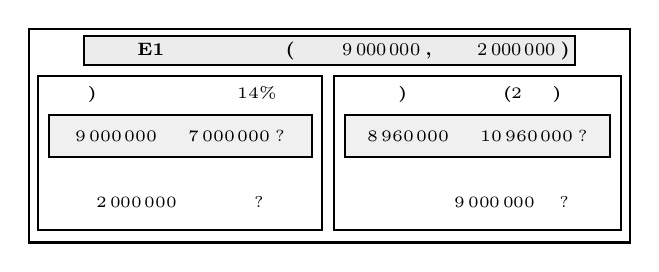
\begin{tikzpicture}[x=0.96cm, y=0.92cm, every node/.style={font=\scriptsize, text=black}]
  \draw[black, line width=0.95pt] (0,0) rectangle (7.95,2.95);
  \node[fill=gray!15, draw=black, line width=0.6pt, inner sep=2pt, font=\fontsize{6.5pt}{8.3pt}\selectfont\bfseries] at (3.975,2.65) {បេសកកម្ម \en{E1}៖ ទិញកុំព្យូទ័របណ្ដាក់ (ថ្លៃដាច់ $9\,000\,000\text{៛}$, កក់មុន $2\,000\,000\text{៛}$)};

  \draw[black, line width=0.8pt] (0.12,0.18) rectangle (3.88,2.30);
  \node[font=\fontsize{5.8pt}{7.5pt}\selectfont\bfseries] at (2.00,2.04) {១) ប្រាក់ដើមសម្រាប់គិតការប្រាក់ $14\%$};
  \draw[black, line width=0.75pt, fill=gray!12] (0.26,1.18) rectangle (3.74,1.76);
  \node[font=\fontsize{5.8pt}{7.5pt}\selectfont] at (2.00,1.47) {$9\,000\,000\text{៛}$ \;ឬ\; $7\,000\,000\text{៛}$?};
  \node[align=center, font=\fontsize{5.7pt}{7.3pt}\selectfont] at (2.00,0.62) {តើគេគិតការប្រាក់លើប្រាក់កក់\\$2\,000\,000\text{៛}$ ដែលបង់រួចដែរឬទេ?};

  \draw[black, line width=0.8pt] (4.04,0.18) rectangle (7.83,2.30);
  \node[font=\fontsize{5.8pt}{7.5pt}\selectfont\bfseries] at (5.935,2.04) {២) ថ្លៃទិញបណ្ដាក់សរុប ($2$ ឆ្នាំ)};
  \draw[black, line width=0.75pt, fill=gray!12] (4.18,1.18) rectangle (7.69,1.76);
  \node[font=\fontsize{5.8pt}{7.5pt}\selectfont] at (5.935,1.47) {$8\,960\,000\text{៛}$ \;ឬ\; $10\,960\,000\text{៛}$?};
  \node[align=center, font=\fontsize{5.7pt}{7.3pt}\selectfont] at (5.935,0.62) {តើថ្លៃទិញបណ្ដាក់សរុបអាចថោក\\ជាងថ្លៃទិញដាច់ $9\,000\,000\text{៛}$ ឬទេ?};
\end{tikzpicture}}

% ២. E2 POE 1 & 2: ខ្សែសង្វាក់ ៤ ជំហាននៃការទិញបណ្ដាក់ (ទំ.៣៨-៤០)
\newcommand{\figPipelineINST}{%
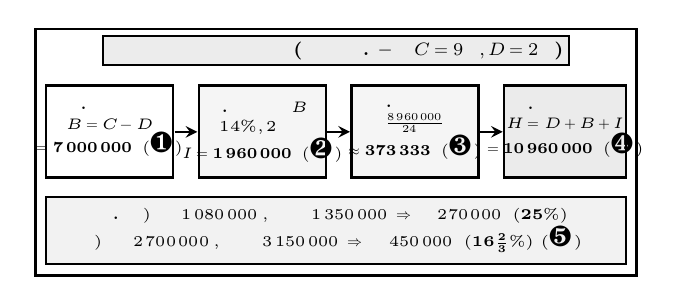
\begin{tikzpicture}[x=0.96cm, y=0.92cm, every node/.style={font=\scriptsize, text=black}]
  \draw[black, line width=0.95pt] (0,0) rectangle (7.95,3.40);
  \node[fill=gray!15, draw=black, line width=0.6pt, inner sep=2pt, font=\fontsize{6.5pt}{8.3pt}\selectfont\bfseries] at (3.975,3.10) {ខ្សែសង្វាក់ ៤ ជំហាននៃការទិញបណ្ដាក់ (កុំព្យូទ័រទំ.៣៨–៣៩៖ $C = 9\text{លាន}, D = 2\text{លាន}$)};

  % 4 pipeline boxes
  \draw[black, line width=0.8pt] (0.14,1.35) rectangle (1.82,2.62);
  \node[align=center, font=\fontsize{5.5pt}{7.1pt}\selectfont] at (0.98,1.98) {\textbf{១. ប្រាក់នៅសល់}\\$B = C - D$\\$=\mathbf{7\,000\,000\text{៛}}$ (\cnum{1})};

  \draw[->, >=stealth, line width=0.85pt] (1.84,1.98) -- (2.14,1.98);

  \draw[black, line width=0.8pt, fill=gray!8] (2.16,1.35) rectangle (3.84,2.62);
  \node[align=center, font=\fontsize{5.5pt}{7.1pt}\selectfont] at (3.00,1.98) {\textbf{២. ការប្រាក់លើ $B$}\\$14\%, 2$ ឆ្នាំ\\$I=\mathbf{1\,960\,000\text{៛}}$ (\cnum{2})};

  \draw[->, >=stealth, line width=0.85pt] (3.86,1.98) -- (4.16,1.98);

  \draw[black, line width=0.8pt, fill=gray!8] (4.18,1.35) rectangle (5.86,2.62);
  \node[align=center, font=\fontsize{5.5pt}{7.1pt}\selectfont] at (5.02,1.98) {\textbf{៣. បង់ប្រចាំខែ}\\$\frac{8\,960\,000}{24\text{ ខែ}}$\\$\approx\mathbf{373\,333\text{៛}}$ (\cnum{3})};

  \draw[->, >=stealth, line width=0.85pt] (5.88,1.98) -- (6.18,1.98);

  \draw[black, line width=0.9pt, fill=gray!16] (6.20,1.35) rectangle (7.81,2.62);
  \node[align=center, font=\fontsize{5.5pt}{7.1pt}\selectfont] at (7.005,1.98) {\textbf{៤. ថ្លៃបណ្ដាក់សរុប}\\$H = D + B + I$\\$=\mathbf{10\,960\,000\text{៛}}$ (\cnum{4})};

  % Summary bar for Practice p.40
  \draw[black, line width=0.75pt, fill=gray!10] (0.14,0.16) rectangle (7.81,1.08);
  \node[align=center, font=\fontsize{5.4pt}{7.0pt}\selectfont] at (3.975,0.62) {\textbf{ទំ.៤០៖} ក) ដាច់ $1\,080\,000\text{៛}$, បណ្ដាក់ $1\,350\,000\text{៛} \Rightarrow$ លើស $270\,000\text{៛}$ ($\mathbf{25\%}$)\\ខ) ដាច់ $2\,700\,000\text{៛}$, បណ្ដាក់ $3\,150\,000\text{៛} \Rightarrow$ លើស $450\,000\text{៛}$ ($\mathbf{16\frac{2}{3}\%}$) (\cnum{5})};
\end{tikzpicture}}

% ៣. E4 Worked Example: គំរូទិញម៉ាស៊ីនបោកខោអាវបណ្ដាក់ (ទំ.៣៩)
\newcommand{\figWasherINST}{%
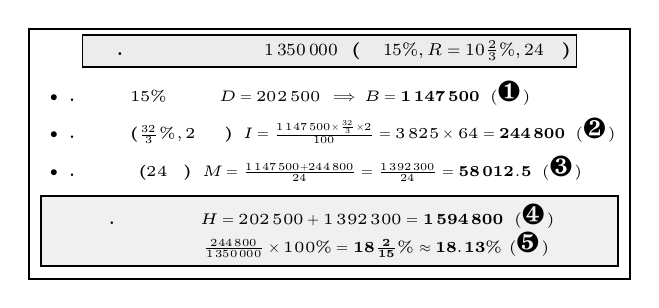
\begin{tikzpicture}[x=0.96cm, y=0.92cm, every node/.style={font=\scriptsize, text=black}]
  \draw[black, line width=0.95pt] (0,0) rectangle (7.95,3.45);
  \node[fill=gray!15, draw=black, line width=0.6pt, inner sep=2pt, font=\fontsize{6.2pt}{8.0pt}\selectfont\bfseries] at (3.975,3.15) {គំរូទំ.៣៩៖ ម៉ាស៊ីនបោកខោអាវថ្លៃដាច់ $1\,350\,000\text{៛}$ (កក់ $15\%, R=10\frac{2}{3}\%, 24$ ខែ)};

  \node[anchor=west, font=\fontsize{5.5pt}{7.2pt}\selectfont] at (0.16,2.56) {$\bullet$ \textbf{១. ប្រាក់កក់ $15\%$ និងនៅសល់៖} $D = 202\,500\text{៛} \implies B = \mathbf{1\,147\,500\text{៛}}$ (\cnum{1})};
  \node[anchor=west, font=\fontsize{5.5pt}{7.2pt}\selectfont] at (0.16,2.04) {$\bullet$ \textbf{២. ការប្រាក់ ($\frac{32}{3}\%, 2$ ឆ្នាំ)៖} $I = \frac{1\,147\,500 \times \frac{32}{3} \times 2}{100} = 3\,825 \times 64 = \mathbf{244\,800\text{៛}}$ (\cnum{2})};
  \node[anchor=west, font=\fontsize{5.5pt}{7.2pt}\selectfont] at (0.16,1.52) {$\bullet$ \textbf{៣. បង់ប្រចាំខែ ($24$ ខែ)៖} $M = \frac{1\,147\,500 + 244\,800}{24} = \frac{1\,392\,300}{24} = \mathbf{58\,012.5\text{៛}}$ (\cnum{3})};

  \draw[black, line width=0.75pt, fill=gray!12] (0.16,0.18) rectangle (7.79,1.14);
  \node[align=center, font=\fontsize{5.6pt}{7.3pt}\selectfont] at (3.975,0.66) {\textbf{៤. ថ្លៃបណ្ដាក់សរុប៖} $H = 202\,500 + 1\,392\,300 = \mathbf{1\,594\,800\text{៛}}$ (\cnum{4})\\ភាគរយលើសថ្លៃទិញដាច់៖ $\frac{244\,800}{1\,350\,000}\times 100\% = \mathbf{18\frac{2}{15}\%} \approx \mathbf{18.13\%}$ (\cnum{5})};
\end{tikzpicture}}

% ៤. E5 Diagnostic Options A-D
\newcommand{\figExitCardsINST}{%
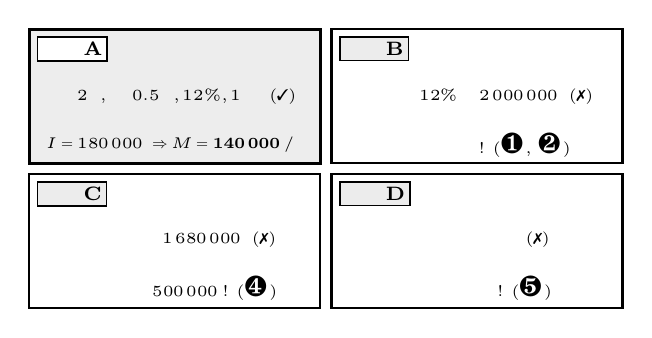
\begin{tikzpicture}[x=0.96cm, y=0.92cm, every node/.style={font=\scriptsize, text=black}]
  \draw[black, line width=1.1pt, fill=gray!14] (0,2.00) rectangle (3.85,3.85);
  \node[anchor=north west, fill=white, draw=black, line width=0.6pt, inner sep=1.8pt] at (0.10,3.75) {\textbf{ជម្រើស \en{A}}};
  \node[font=\fontsize{5.6pt}{7.3pt}\selectfont] at (1.925,2.92) {ដាច់ $2\text{លាន}$, កក់ $0.5\text{លាន}, 12\%, 1\text{ឆ្នាំ}$ (\ding{51})};
  \node[font=\fontsize{5.6pt}{7.3pt}\selectfont] at (1.925,2.25) {$I=180\,000\text{៛} \Rightarrow M=\mathbf{140\,000\text{៛}}$/ខែ};

  \draw[black, line width=0.9pt] (4.00,2.00) rectangle (7.85,3.85);
  \node[anchor=north west, fill=gray!15, draw=black, line width=0.6pt, inner sep=1.8pt] at (4.10,3.75) {\textbf{ជម្រើស \en{B}}};
  \node[font=\fontsize{5.6pt}{7.3pt}\selectfont] at (5.925,2.92) {គិតការប្រាក់ $12\%$ លើ $2\,000\,000\text{៛}$ (\ding{55})};
  \node[font=\fontsize{5.6pt}{7.3pt}\selectfont] at (5.925,2.25) {ភ្លេចដកប្រាក់កក់ចេញសិន! (\cnum{1}, \cnum{2})};

  \draw[black, line width=0.9pt] (0,0) rectangle (3.85,1.85);
  \node[anchor=north west, fill=gray!15, draw=black, line width=0.6pt, inner sep=1.8pt] at (0.10,1.75) {\textbf{ជម្រើស \en{C}}};
  \node[font=\fontsize{5.6pt}{7.3pt}\selectfont] at (1.925,0.95) {ថ្លៃបណ្ដាក់សរុបស្មើ $1\,680\,000\text{៛}$ (\ding{55})};
  \node[font=\fontsize{5.6pt}{7.3pt}\selectfont] at (1.925,0.28) {ភ្លេចបូកប្រាក់កក់ $500\,000\text{៛}$! (\cnum{4})};

  \draw[black, line width=0.9pt] (4.00,0) rectangle (7.85,1.85);
  \node[anchor=north west, fill=gray!15, draw=black, line width=0.6pt, inner sep=1.8pt] at (4.10,1.75) {\textbf{ជម្រើស \en{D}}};
  \node[font=\fontsize{5.6pt}{7.3pt}\selectfont] at (5.925,0.95) {ភាគរយលើស ចែកនឹងថ្លៃបណ្ដាក់ (\ding{55})};
  \node[font=\fontsize{5.6pt}{7.3pt}\selectfont] at (5.925,0.28) {ត្រូវចែកនឹងថ្លៃទិញដាច់! (\cnum{5})};
\end{tikzpicture}}

\begin{document}
\fontsize{10pt}{15.2pt}\selectfont

% -------------------- ក្បាលកិច្ចតែងការ --------------------
\begin{center}
  {\muol\fontsize{11pt}{16pt}\selectfont ព្រះរាជាណាចក្រកម្ពុជា}\\[2pt]
  {\muol\fontsize{10pt}{15pt}\selectfont ជាតិ សាសនា ព្រះមហាក្សត្រ}\\[1pt]
  \khmflourish
\end{center}

\vspace{-24pt}
{\muol\fontsize{9.5pt}{12.5pt}\selectfont
មន្ទីរអប់រំ យុវជន និងកីឡា ខេត្តកំពង់ធំ\\
ការិយាល័យអប់រំ យុវជន និងកីឡា ស្រុកកំពង់ស្វាយ\\
អនុវិទ្យាល័យព្រះក្រសាំង}

\vspace{1pt}
\begin{center}
  {\muol\fontsize{10pt}{14pt}\selectfont កិច្ចតែងការបង្រៀន}
\end{center}
\vspace{0pt}

% -------------------- ព័ត៌មានទូទៅ --------------------
{\renewcommand{\arraystretch}{0.98}
\hspace*{3.1cm}%
\begin{tabular}{@{}l l L{11.0cm}@{}}
  - \hspace{0.35cm} មុខវិជ្ជា & : & គណិតវិទ្យា ថ្នាក់ទី៨ (ពីជគណិត) \\
  - \hspace{0.35cm} ចំណងជើងមេរៀន & : & មេរៀនទី៣៖ ទំហំសមាមាត្រ និងភាគរយ \\
  - \hspace{0.35cm} ចំណងជើងរង & : & ២.៧. ការទិញបណ្ដាក់ និងសង្ខេបមេរៀនទី៣ (ទំ.៣៨–៤០ និងលំហាត់ \#19 ទំ.៤២) \\
  - \hspace{0.35cm} រយៈពេល & : & ១ ម៉ោងសិក្សា (៥០ នាទី — ម៉ោងបញ្ចប់មេរៀនទី៣) \\
  - \hspace{0.35cm} បង្រៀនដោយ & : & ហុក ប៊ុនថែន \\
  - \hspace{0.35cm} កាលបរិច្ឆេទ & : & ថ្ងៃព្រហស្បតិ៍ ទី៣ ខែធ្នូ ឆ្នាំ២០២៦ \\
\end{tabular}

\vspace{2pt}

% -------------------- I. វត្ថុបំណង --------------------
\textbf{I.} {\muol វត្ថុបំណង}\\[1pt]
\hspace*{0.55cm}%
\begin{tabular}{@{}l l L{14.2cm}@{}}
  \wcirc \hspace{0.25cm} វិជ្ជាសម្បទា & : & សិស្សប្រាប់អត្ថន័យនៃប្រាក់កក់ ប្រាក់នៅសល់ ប្រាក់បង់ប្រចាំខែ និងថ្លៃទិញបណ្ដាក់សរុប ព្រមទាំងសំយោគរូបមន្តគោលទាំងអស់នៃមេរៀនទី៣បានត្រឹមត្រូវ ។ \\
  \wcirc \hspace{0.25cm} បំណិនសម្បទា & : & សិស្សគណនាប្រាក់នៅសល់ ប្រាក់បង់ប្រចាំខែ ថ្លៃទិញបណ្ដាក់សរុប និងភាគរយលើសពីថ្លៃទិញដាច់ (ទំ.៣៨–៤០) ដោយដៃលើសន្លឹកកិច្ចការបានត្រឹមត្រូវ ។ \\
  \wcirc \hspace{0.25cm} ចរិយាសម្បទា & : & សិស្សមានស្មារតីពិចារណាល្អិតល្អន់មុនសម្រេចចិត្តទិញទំនិញបង់រំលស់ ដោយចេះប្រៀបធៀបថ្លៃទិញដាច់ និងថ្លៃទិញបណ្ដាក់ក្នុងជីវភាពរស់នៅជាក់ស្ដែង ។ \\
\end{tabular}

\vspace{2pt}

% -------------------- II. សម្ភារៈឧបទេស --------------------
\textbf{II.} {\muol សម្ភារៈឧបទេស}\\[1pt]
\hspace*{0.55cm}$\bullet$ \hspace{0.35cm} សៀវភៅសិក្សាគោលគណិតវិទ្យាថ្នាក់ទី៨ (ទំ.៣៨–៤២) ក្ដារខៀន ដីស និងសន្លឹកកិច្ចការសិស្ស ស-ខ្មៅ (\en{Worksheet\_INST} ទំព័រ ១–២ គ្មានស្លាយ \en{LCD})

\vspace{2pt}

% -------------------- III. វិធីសាស្រ្តបង្រៀន --------------------
\textbf{III.} {\muol វិធីសាស្រ្តបង្រៀន}\\[1pt]
\hspace*{0.45cm}%
\begin{tabular}{@{}l l L{14.85cm}@{}}
  $\bullet$ \hspace{0.25cm} គោលវិធី & : & សិស្សមជ្ឈមណ្ឌល (បង្រៀនតាមសន្លឹកកិច្ចការស៊ើបអង្កេត និងក្ដារខៀន គ្មាន \en{LCD}) \\
  $\bullet$ \hspace{0.25cm} យុទ្ធវិធីបង្រៀន & : & គំរូ \en{5Es} រួមបញ្ចូលខ្សែសង្វាក់ប្រាក់នៅសល់ ៤ ជំហាន និងតារាងប្រៀបធៀបទិញដាច់-ទិញបណ្ដាក់ \\
\end{tabular}
}

\vspace{2pt}

% -------------------- IV. ដំណើរការបង្រៀន --------------------
\textbf{IV.} {\muol ដំណើរការបង្រៀន}

\vspace{1pt}

\renewcommand{\arraystretch}{1.15}
\begin{longtable}{|L{5.50cm}|L{7.90cm}|L{4.80cm}|}
\hline
\rowcolor{headgray}
\multicolumn{1}{|c|}{\muol សកម្មភាពគ្រូ} &
\multicolumn{1}{c|}{\muol ខ្លឹមសារមេរៀន} &
\multicolumn{1}{c|}{\muol សកម្មភាពសិស្ស} \\
\hline
\endfirsthead
\hline
\endhead
\hline
\endfoot
\hline
\endlastfoot

% ==================== ជំហានទី១ (2min) ====================
\stepheader{ជំហានទី១ \enbf{(}រដ្ឋបាលថ្នាក់\enbf{)}}
$\bullet$ ពិនិត្យអវត្តមាន អនាម័យ និងសណ្ដាប់ធ្នាប់ថ្នាក់រៀន
&
$\bullet$ រដ្ឋបាលថ្នាក់ និងការរៀបចំដៃគូសិក្សា
&
$\circ$ ប្រធានថ្នាក់រាយការណ៍អវត្តមាន \\[3pt]

$\bullet$ ចែក \textbf{សន្លឹកកិច្ចការសិស្ស (\en{Worksheet\_INST})} ម្នាក់ ១ សន្លឹក (ផ្កាប់ទុកសិន)
&
$\bullet$ សន្លឹកកិច្ចការសិស្ស ស-ខ្មៅ (\en{Worksheet\_INST} ទំព័រ ១–២)
&
$\circ$ ទទួលសន្លឹកកិច្ចការ និងត្រៀមសម្ភារៈសរសេរ \\
\hline

% ==================== ជំហានទី២ (9min: <=3 + 3 + E1 3) ====================
\stepheader{ជំហានទី២ \enbf{(}កិច្ចការផ្ទះ \enbf{+} ទំនាក់ទំនងមេរៀនថ្មី\enbf{)}}
\ditem \textbf{កំណែកិច្ចការផ្ទះ ($\le 3\unit{min}$)} \timenote{(កុំសរសេរវែង)} \par
$\bullet$ ហៅសិស្ស ២ នាក់ឡើងសរសេរចម្លើយលំហាត់ \#17 ក, ខ និង \#18 (ទំ.៤២) លើក្ដារខៀន
&
{\centering\redsub{កំណែកិច្ចការផ្ទះមេរៀន ២.៦ (ទំ.៤២ \#17 ក, ខ និង \#18)}\par} \par
$\bullet$ \textbf{\#17 ក-ខ៖} គណនាការប្រាក់សមាសតាមតារាងបង្វិលប្រាក់ដើម ($P_{k+1} = P_k + I_k$) \par
$\bullet$ \textbf{\#18៖} គណនាការប្រាក់សមាសគិតរាល់កន្លះឆ្នាំម្ដង ($T = \frac{1}{2}$ ឆ្នាំក្នុងមួយគ្រា)
&
$\circ$ ផ្ទៀងផ្ទាត់ និងកែតម្រូវចម្លើយក្នុងសៀវភៅកិច្ចការផ្ទះ \\[3pt]

\ditem \textbf{រំលឹកមេរៀនទាក់ទង (3min)} \par
$\bullet$ សួររហ័ស៖ ម៉ាស៊ីនថ្លៃ $1\,000\,000\text{៛}$ បើគេកក់មុន $20\%$ តើប្រាក់នៅសល់ស្មើប៉ុន្មាន?
&
{\centering\redsub{រំលឹកប្រាក់កក់ និងការប្រាក់សាមញ្ញ}\par} \par
$\bullet$ ប្រាក់កក់ $= 200\,000\text{៛} \implies$ ប្រាក់នៅសល់ $= 1\,000\,000 - 200\,000 = \mathbf{800\,000\text{៛}}$
&
$\circ$ គណនារហ័សថាប្រាក់នៅសល់ស្មើ $800\,000\text{៛}$ \\[3pt]

$\bullet$ សួររហ័សបន្ត៖ ចុះបើគិតការប្រាក់សាមញ្ញ $10\%$/ឆ្នាំ លើប្រាក់នៅសល់ $800\,000\text{៛}$ រយៈពេល $2$ ឆ្នាំ ស្មើប៉ុន្មាន?
&
$\bullet$ ការប្រាក់ $I = \frac{800\,000 \times 10 \times 2}{100} = \mathbf{160\,000\text{៛}}$
&
$\circ$ ឆ្លើយរហ័សថាស្មើ $160\,000\text{៛}$ \\[3pt]

\fiveE{E1 - Engage (3min)} \timenote{(កុំទាន់ផ្ដល់ចម្លើយ)} \par
\ditem \textbf{«បេសកកម្មទិញកុំព្យូទ័របណ្ដាក់ (ទំ.៣៨–៣៩)»} \par
$\bullet$ ឱ្យសិស្សបើកសន្លឹកកិច្ចការទំព័រ ១ គូសធីកទស្សន៍ទាយលើសំណួរ ២
&
{\centering\redsub{បេសកកម្ម E1៖ អន្ទាក់ការប្រាក់លើប្រាក់កក់ និងថ្លៃបណ្ដាក់សរុប}\par} \par
$\bullet$ \textbf{សំណួរ ១ (ទំ.៣៨)៖} កុំព្យូទ័រថ្លៃដាច់ $9\,000\,000\text{៛}$ កក់មុន $2\,000\,000\text{៛}$ — តើហាងគិតការប្រាក់ $14\%$ លើ $9\,000\,000\text{៛}$ ឬលើ $7\,000\,000\text{៛}$? \par
$\bullet$ \textbf{សំណួរ ២៖} តើថ្លៃទិញបណ្ដាក់សរុបស្មើ $8\,960\,000\text{៛}$ ឬ $10\,960\,000\text{៛}$?
&
$\circ$ គូសធីកទស្សន៍ទាយលើសន្លឹកកិច្ចការទំព័រ ១ \\[3pt]

&
\cfig{\figEngageINST}
& \\[3pt]

$\bullet$ ស្រង់ចំនួនដៃសិស្សកត់លើក្ដារខៀន (មិនទាន់ប្រាប់ចម្លើយត្រូវ)
&
$\bullet$ ស្ថិតិទស្សន៍ទាយ៖ គិតការប្រាក់លើ $9\text{លាន}$ ទល់នឹង $7\text{លាន}$
&
$\circ$ លើកដៃបង្ហាញការទស្សន៍ទាយ \\
\hline

% ==================== ជំហានទី៣ (17min: E2 11m + E3 6m) ====================
\stepheader{ជំហានទី៣ \enbf{(}ខ្លឹមសារមេរៀនថ្មី\enbf{)}}
\fiveE{E2 - Explore (11min)} \par
$\bullet$ សរសេរចំណងជើងរងលើក្ដារខៀន
&
\textbf{២.៧. ការទិញបណ្ដាក់ និងសង្ខេបមេរៀនទី៣} (សៀវភៅពុម្ព ទំ.៣៨–៤០)
&
$\circ$ កត់ចំណងជើងចូលសៀវភៅ \\[3pt]

\ditem \textbf{សកម្មភាព ១៖ ខ្សែសង្វាក់ ៤ ជំហាននៃការទិញកុំព្យូទ័របណ្ដាក់ \en{POE 1} (5min, ទំ.៣៨–៣៩)} \par
$\bullet$ ឱ្យដៃគូបំពេញតារាង ៤ ជំហាននៃការទិញកុំព្យូទ័របណ្ដាក់ ($C = 9\text{លាន}, D = 2\text{លាន}, R = 14\%, 2$ ឆ្នាំ) លើសន្លឹកកិច្ចការ
&
{\centering\textbf{សកម្មភាព ១ (\en{POE 1})៖ ទិញកុំព្យូទ័របណ្ដាក់ (ទំ.៣៨–៣៩)}\par} \par
$\bullet$ ប្រាក់នៅសល់ $B = 9\,000\,000 - 2\,000\,000 = \mathbf{7\,000\,000\text{៛}}$ \par
$\bullet$ ការប្រាក់ $I = \frac{7\,000\,000\times 14\times 2}{100} = \mathbf{1\,960\,000\text{៛}} \implies$ រំលស់សរុប $8\,960\,000\text{៛}$ \par
$\bullet$ ប្រចាំខែ ($24$ ខែ) $\approx \mathbf{373\,333.33\text{៛}}$ ; ថ្លៃបណ្ដាក់សរុប $= \mathbf{10\,960\,000\text{៛}}$
&
$\circ$ រកឃើញថាការប្រាក់គិតតែលើប្រាក់នៅសល់ $7\text{លាន}$ ហើយថ្លៃបណ្ដាក់សរុបត្រូវបូកប្រាក់កក់ចូលវិញ! \\[3pt]

\ditem \textbf{សកម្មភាព ២៖ តារាងប្រៀបធៀបទិញដាច់ ទល់នឹង ទិញបណ្ដាក់ \en{POE 2} (6min, ទំ.៤០)} \par
$\bullet$ ឱ្យដៃគូបំពេញតារាងប្រតិបត្តិទំ.៤០ (ក និង ខ) ដើម្បីរកថ្លៃបណ្ដាក់សរុប និងភាគរយលើសដាច់
&
{\centering\textbf{សកម្មភាព ២ (\en{POE 2})៖ ប្រតិបត្តិទំ.៤០ (ក និង ខ)}\par} \par
$\bullet$ \textbf{ក.} ដាច់ $1\,080\,000\text{៛}$ ; បណ្ដាក់ $= 150\,000 + 10\times 120\,000 = \mathbf{1\,350\,000\text{៛}}$ \par
$\implies$ លើស $270\,000\text{៛} \implies \% = \frac{270\,000}{1\,080\,000}\times 100\% = \mathbf{25\%}$ \par
$\bullet$ \textbf{ខ.} ដាច់ $2\,700\,000\text{៛}$ ; បណ្ដាក់ $= 450\,000 + 12\times 225\,000 = \mathbf{3\,150\,000\text{៛}}$ ($\mathbf{16\frac{2}{3}\%}$)
&
$\circ$ គណនាថ្លៃបណ្ដាក់សរុប និងរកឃើញថាភាគរយលើសត្រូវធៀបនឹងថ្លៃទិញដាច់ ($100\%$) \\[3pt]

&
\cfig{\figPipelineINST}
& \\[3pt]

% --- E3 Explain (6min) ---
\fiveE{E3 - Explain (6min)} \par
$\bullet$ ឱ្យសិស្សបង្គុំប្រអប់ \textbf{ប្រាក់នៅសល់ និងការប្រាក់ទិញបណ្ដាក់} (ផ្នែកទី២)
&
$\bullet$ \textbf{ប្រាក់នៅសល់ត្រូវបង់រំលស់៖} $B = \text{ថ្លៃទិញដាច់ } C - \text{ប្រាក់កក់ } D$ \par
$\bullet$ \textbf{ការប្រាក់ទិញបណ្ដាក់៖} $I = \frac{B \cdot R \cdot T}{100}$ (គិតតែលើប្រាក់នៅសល់ $B$) ។
&
$\circ$ បំពេញប្រអប់រូបមន្តប្រាក់នៅសល់ និងការប្រាក់លើសន្លឹកកិច្ចការ \\[3pt]

$\bullet$ ឱ្យសិស្សបង្គុំប្រអប់ \textbf{ប្រាក់បង់ប្រចាំខែ ថ្លៃបណ្ដាក់សរុប និងភាគរយលើស}
&
$\bullet$ \textbf{ប្រាក់បង់ប្រចាំខែ ($n$ ខែ)៖} $M = \frac{B + I}{n}$ \;;\; \textbf{ថ្លៃបណ្ដាក់សរុប៖} $H = D + nM = C + I$ \par
$\bullet$ \textbf{ភាគរយលើសពីថ្លៃទិញដាច់៖} $\%\text{លើស} = \frac{H - C}{C} \times 100\%$ ។
&
$\circ$ បំពេញប្រអប់រូបមន្តប្រាក់ប្រចាំខែ និងថ្លៃសរុបលើសន្លឹកកិច្ចការ \\[3pt]

$\bullet$ សង្ខេប \textbf{ធនាគារហេតុផល \cnum{1}--\cnum{3}} អំពីប្រាក់នៅសល់ ការប្រាក់ និងប្រាក់ប្រចាំខែ
&
\textbf{ធនាគារហេតុផល \en{B\&W} (\cnum{1}--\cnum{5})៖} \par
\cnum{1} ប្រាក់នៅសល់៖ $B = \text{ថ្លៃទិញដាច់} - \text{ប្រាក់កក់}$ \par
\cnum{2} ការប្រាក់បណ្ដាក់៖ គិតតែលើប្រាក់នៅសល់ ($I = \frac{BRT}{100}$) មិនគិតលើប្រាក់កក់ទេ \par
\cnum{3} ប្រាក់បង់ប្រចាំខែ៖ $M = \frac{\text{ប្រាក់នៅសល់ } B + \text{ការប្រាក់ } I}{\text{ចំនួនខែ } n}$
&
$\circ$ ផ្ទៀងផ្ទាត់ហេតុផល \cnum{1}--\cnum{3} លើសន្លឹកកិច្ចការ \\[3pt]

$\bullet$ សង្ខេប \textbf{ធនាគារហេតុផល \cnum{4}--\cnum{5}} សម្រាប់ថ្លៃទិញបណ្ដាក់សរុប និងភាគរយលើស
&
\cnum{4} ថ្លៃទិញបណ្ដាក់សរុប៖ $H = \text{ប្រាក់កក់} + (\text{ប្រចាំខែ} \times n) = \text{ថ្លៃទិញដាច់} + I$ \par
\cnum{5} ភាគរយថ្លៃលើស៖ $\%\text{លើស} = \frac{H - \text{ថ្លៃទិញដាច់}}{\text{ថ្លៃទិញដាច់}} \times 100\%$ (គោលថ្លៃដាច់ $100\%$)
&
$\circ$ ផ្ទៀងផ្ទាត់ហេតុផល \cnum{4}--\cnum{5} លើសន្លឹកកិច្ចការ \\
\hline

% ==================== ជំហានទី៤ (20min: E4 10m + E5 10m) ====================
\stepheader{ជំហានទី៤ \enbf{(}ពង្រីកចំណេះដឹង និងវាយតម្លៃ\enbf{)}}
\fiveE{E4 - Elaborate (10min)} \par
\ditem \textbf{លំហាត់គំរូ៖ ទិញម៉ាស៊ីនបោកខោអាវបណ្ដាក់ (ទំ.៣៩ — ផ្នែកទី៣)} \par
$\bullet$ ដឹកនាំដោះស្រាយ \textbf{គំរូទំ.៣៩ (ថ្លៃដាច់ $1\,350\,000\text{៛}$, កក់មុន $15\%$, ការប្រាក់ $10\frac{2}{3}\%$/ឆ្នាំ រយៈពេល $2$ ឆ្នាំ $= 24$ ខែ)}
&
{\muol លំហាត់គំរូ} \textbf{(ទំ.៣៩ — ម៉ាស៊ីនបោកខោអាវថ្លៃដាច់ $1\,350\,000\text{៛}$)៖} \par
$\bullet$ ប្រាក់កក់ $15\%$៖ $D = 202\,500\text{៛} \implies B = \mathbf{1\,147\,500\text{៛}}$ (\cnum{1}) \par
$\bullet$ ការប្រាក់ ($R = \frac{32}{3}\%, T = 2$)៖ $I = \frac{1\,147\,500\times \frac{32}{3}\times 2}{100} = \mathbf{244\,800\text{៛}}$ (\cnum{2}) \par
$\bullet$ បង់ប្រចាំខែ ($24$ ខែ)៖ $M = \frac{1\,392\,300}{24} = \mathbf{58\,012.5\text{៛}}$ (\cnum{3}) \par
$\bullet$ ថ្លៃបណ្ដាក់សរុប៖ $H = \mathbf{1\,594\,800\text{៛}}$ (លើសដាច់ $\mathbf{18\frac{2}{15}\%}$) (\cnum{4}, \cnum{5})
&
$\circ$ បំពេញតារាងគណនាទាំង ៤ ជំហានដោយដៃលើសន្លឹកកិច្ចការ \\[3pt]

&
\cfig{\figWasherINST}
& \\[3pt]

$\bullet$ សួរសំណួរឆ្លុះបញ្ចាំង \textbf{\en{EIA Looking-Back} (៣០ វិនាទី)}
&
\textbf{\en{EIA Looking-Back}៖} «បើអ្នកបង្កើនប្រាក់កក់ដំបូងឱ្យកាន់តែច្រើន តើប្រាក់ការដែលត្រូវបង់នឹងកើនឡើង ឬថយចុះ?»
&
$\circ$ ឆ្លើយ៖ «ថយចុះ ព្រោះប្រាក់នៅសល់ $B$ កាន់តែតូច!» \\[3pt]

% --- E5 Evaluate (10min) ---
\fiveE{E5 - Evaluate (10min)} \par
\ditem \textbf{ហ្វឹកហាត់ជាដៃគូលើ «ការទិញបណ្ដាក់ និងសំយោគមេរៀនទី៣» (6min — ផ្នែកទី៤-ក)} \par
$\bullet$ ឱ្យដៃគូធ្វើ \textbf{លំហាត់ ១ (កង់អគ្គិសនីថ្លៃដាច់ $2\,000\,000\text{៛}$, កក់ $25\%$, អត្រា $12\%$/ឆ្នាំ រយៈពេល $12$ ខែ)}
&
{\muol លំហាត់ប្រតិបត្តិ} \textbf{(អនុវត្តការទិញបណ្ដាក់ និងសំយោគមេរៀនទី៣)៖} \par
$\bullet$ \textbf{១) កង់អគ្គិសនី ($C=2\,000\,000\text{៛}$, កក់ $25\% = 500\,000\text{៛}$)៖} \par
$B = 1\,500\,000\text{៛} \implies I = \frac{1\,500\,000\times 12\times 1}{100} = 180\,000\text{៛}$ (\cnum{1}, \cnum{2}) \par
$\implies M = \frac{1\,680\,000}{12} = \mathbf{140\,000\text{៛}}$/ខែ ; $H = \mathbf{2\,180\,000\text{៛}}$ (\cnum{3}, \cnum{4})
&
$\circ$ គណនាប្រាក់នៅសល់ ការប្រាក់ ប្រាក់ប្រចាំខែ និងថ្លៃសរុប \\[3pt]

$\bullet$ ឱ្យដៃគូធ្វើ \textbf{លំហាត់ ២ (សំយោគរូបមន្តគោលទាំង ៤ ក្រុមនៃមេរៀនទី៣ ទំ.៤០)} រួចប្ដូរសន្លឹកផ្ទៀង (\en{Pause-Review})
&
$\bullet$ \textbf{២) សំយោគមេរៀនទី៣ (ទំ.៤០)៖} \par
សមាមាត្រស្រប $\frac{y}{x} = k$ \en{|} សមាមាត្រច្រាស $x \cdot y = k$ \par
ការប្រាក់សាមញ្ញ $I = \frac{PRT}{100}$ \en{|} សមាស $P_{k+1} = P_k + I_k$
&
$\circ$ បំពេញផែនទីសំយោគរូបមន្តមេរៀនទី៣ និងផ្ទៀងជាមួយដៃគូ \\[3pt]

$\bullet$ បិទបេសកកម្ម \en{E1} និងរំលឹកអន្ទាក់ទាំងពីរនៃការទិញបណ្ដាក់
&
$\bullet$ \textbf{បិទបេសកកម្ម \en{E1}៖} គិតការប្រាក់តែលើប្រាក់នៅសល់ $\mathbf{7\,000\,000\text{៛}}$ ហើយថ្លៃបណ្ដាក់សរុបគឺ $\mathbf{10\,960\,000\text{៛}}$ (បូកប្រាក់កក់ចូលវិញ) ។
&
$\circ$ ផ្ទៀងចម្លើយ \en{E1} និងកត់ចំណាំលើសន្លឹកកិច្ចការ \\[3pt]

$\bullet$ ឱ្យសិស្សវិនិច្ឆ័យ \textbf{ជម្រើស \en{A--D}} លើសន្លឹកកិច្ចការ (ផ្នែកទី៤-ខ)
&
$\bullet$ \textbf{វិនិច្ឆ័យជម្រើស \en{A--D} លើសន្លឹកកិច្ចការ៖} ជ្រើសជម្រើសត្រូវ \en{A} និងដាក់លេខហេតុផលនៃជម្រើសខុស
&
$\circ$ គូសវង់ជម្រើសត្រូវ \en{A} និងដាក់លេខហេតុផល \cnum{1}--\cnum{5} \\[3pt]

&
\cfig{\figExitCardsINST}
& \\[3pt]

$\bullet$ ពិនិត្យរហ័សលើសំបុត្រចេញនៅបាតសន្លឹកកិច្ចការ (៦០ វិនាទី)
&
$\bullet$ \textbf{\en{Exit Check}៖} ទូរស័ព្ទថ្លៃដាច់ $800\,000\text{៛}$ កក់ $200\,000\text{៛}$ និងបង់ $10$ ខែ $\times 72\,000\text{៛}$៖ ១) $H = \mathbf{920\,000\text{៛}}$ ; ២) លើសដាច់ $\mathbf{15\%}$ ។
&
$\circ$ បំពេញសំបុត្រចេញដោយខ្លួនឯង \\
\hline

% ==================== ជំហានទី៥ (<=2min) ====================
\stepheader{ជំហានទី៥ \enbf{(}កិច្ចការផ្ទះ \enbf{+} បណ្ដាំផ្ញើ\enbf{)}}
\timenote{ចំណាយពេលឱ្យតិចបំផុតកុំឱ្យលើស 2min} \par
$\bullet$ ណែនាំកិច្ចការផ្ទះនៅបាតសន្លឹកកិច្ចការ (សៀវភៅពុម្ព ទំ.៤២ លំហាត់ \#19 និងរំលឹកមេរៀនទី៣ទាំងមូល)
&
{\centering{\muol កិច្ចការផ្ទះ} \textbf{(សៀវភៅគោល ទំ.៤២ លំហាត់ \#19 និងសង្ខេបទំ.៤០–៤២)៖}\par} \par
$\bullet$ \textbf{លំហាត់ \#19 (ទំ.៤២)៖} គណនាប្រាក់នៅសល់ ប្រាក់បង់ប្រចាំខែ និងថ្លៃទិញបណ្ដាក់សរុប \par
$\bullet$ \textbf{រំលឹកសំយោគមេរៀនទី៣៖} ធ្វើលំហាត់ជ្រើសរើសបន្ថែមទំ.៤១–៤២ ដើម្បីត្រៀមប្រឡងបញ្ចប់មេរៀនទី៣
&
$\circ$ កត់ចំណាំលំហាត់ \#19 និងរំលឹកសង្ខេបមេរៀនទី៣ទាំងមូល \\[3pt]

$\bullet$ ផ្ដាំផ្ញើឱ្យអានមុន \textbf{មេរៀនទី៤៖ កន្សោមពីជគណិត (ទំ.៤៣)} សម្រាប់ម៉ោងក្រោយ
&
$\bullet$ \textbf{មេរៀនបន្ទាប់៖} អានមុន \textbf{មេរៀនទី៤៖ កន្សោមពីជគណិត (ទំ.៤៣)} ។
&
$\circ$ កត់ចំណាំមេរៀនបន្ទាប់ និងជម្រាបលាគ្រូ \\
\end{longtable}

\vspace{6pt}
\hfill
\begin{minipage}{10.5cm}
  {\centering
    ថ្ងៃព្រហស្បតិ៍ ៩រោច ខែកត្តិក ឆ្នាំមមី អដ្ឋស័ក ពុទ្ធសករាជ ២៥៧០\\[2pt]
    កំពង់ស្វាយ, ថ្ងៃទី៣ ខែធ្នូ ឆ្នាំ២០២៦\\[3pt]
    {\muol គ្រូបង្រៀន}\par}
  \vspace{28pt}
  \hfill{\muol ហុក ប៊ុនថែន}\hspace*{1.4cm}
\end{minipage}

\end{document}
